\documentclass[crop,tikz]{standalone}
\usepackage{tikz}
\usepackage{xcolor}
\usetikzlibrary{backgrounds,calc,shapes,arrows,decorations.pathreplacing,decorations.markings,patterns,positioning,3d}

% Define colors
\definecolor{edgecolor}{RGB}{64, 64, 140}
\definecolor{nodecolor}{RGB}{180, 60, 60}
\definecolor{fillcolor2}{RGB}{220, 140, 140}
\definecolor{fillcolor3}{RGB}{140, 140, 220}
\definecolor{fillcolor4}{RGB}{140, 220, 140}

\begin{document}
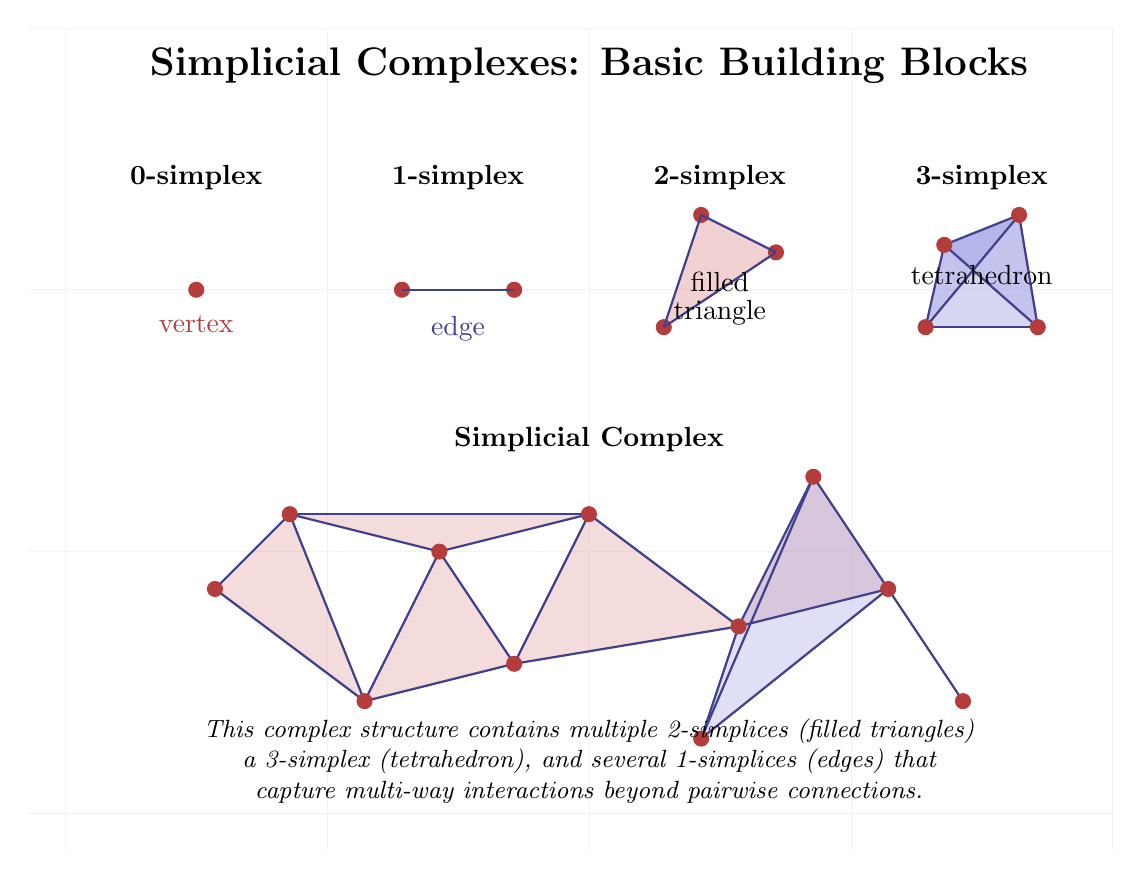
\begin{tikzpicture}[scale=0.95]
  % Grid for organization
  \draw[step=3.5cm, black!5, very thin] (-0.5,-0.5) grid (14,10.5);

  % Title
  \node[font=\Large\bfseries] at (7,10) {Simplicial Complexes: Basic Building Blocks};

  % 0-simplex (Point)
  \node[font=\bfseries] at (1.75,8.5) {0-simplex};
  \filldraw[nodecolor] (1.75,7) circle (0.1) node[below=0.2cm] {vertex};

  % 1-simplex (Edge)
  \node[font=\bfseries] at (5.25,8.5) {1-simplex};
  \filldraw[nodecolor] (4.5,7) circle (0.1);
  \filldraw[nodecolor] (6,7) circle (0.1);
  \draw[thick, edgecolor] (4.5,7) -- (6,7) node[midway, below=0.2cm] {edge};

  % 2-simplex (Filled triangle)
  \node[font=\bfseries] at (8.75,8.5) {2-simplex};
  \filldraw[fillcolor2, opacity=0.4] (8,6.5) -- (9.5,7.5) -- (8.5,8) -- cycle;
  \filldraw[nodecolor] (8,6.5) circle (0.1);
  \filldraw[nodecolor] (9.5,7.5) circle (0.1);
  \filldraw[nodecolor] (8.5,8) circle (0.1);
  \draw[thick, edgecolor] (8,6.5) -- (9.5,7.5);
  \draw[thick, edgecolor] (9.5,7.5) -- (8.5,8);
  \draw[thick, edgecolor] (8.5,8) -- (8,6.5);
  \node at (8.75,7.1) {filled};
  \node at (8.75,6.7) {triangle};

  % 3-simplex (Tetrahedron) with perspective
  \node[font=\bfseries] at (12.25,8.5) {3-simplex};

  % Tetrahedron coordinates with perspective
  \coordinate (A) at (11.5,6.5);
  \coordinate (B) at (13,6.5);
  \coordinate (C) at (12.75,8);
  \coordinate (D) at (11.75,7.6);

  % Back faces (drawn first)
  \filldraw[fillcolor3, opacity=0.2] (A) -- (B) -- (C) -- cycle;
  \filldraw[fillcolor3, opacity=0.2] (A) -- (B) -- (D) -- cycle;

  % Front faces
  \filldraw[fillcolor3, opacity=0.4] (A) -- (C) -- (D) -- cycle;
  \filldraw[fillcolor3, opacity=0.4] (B) -- (C) -- (D) -- cycle;

  % Edges
  \draw[thick, edgecolor] (A) -- (B);
  \draw[thick, edgecolor] (A) -- (C);
  \draw[thick, edgecolor] (A) -- (D);
  \draw[thick, edgecolor] (B) -- (C);
  \draw[thick, edgecolor] (B) -- (D);
  \draw[thick, edgecolor] (C) -- (D);

  % Vertices
  \filldraw[nodecolor] (A) circle (0.1);
  \filldraw[nodecolor] (B) circle (0.1);
  \filldraw[nodecolor] (C) circle (0.1);
  \filldraw[nodecolor] (D) circle (0.1);

  \node at (12.25,7.2) {tetrahedron};

  % Complex simplicial complex example
  \node[font=\bfseries] at (7,5) {Simplicial Complex};

  % Create a complex simplicial complex with various dimensions
  % Define vertices
  \coordinate (V1) at (2,3);
  \coordinate (V2) at (4,1.5);
  \coordinate (V3) at (6,2);
  \coordinate (V4) at (5,3.5);
  \coordinate (V5) at (3,4);
  \coordinate (V6) at (7,4);
  \coordinate (V7) at (9,2.5);
  \coordinate (V8) at (11,3);
  \coordinate (V9) at (10,4.5);
  \coordinate (V10) at (8.5,1);
  \coordinate (V11) at (12,1.5);

  % Draw filled triangles (2-simplices)
  \filldraw[fillcolor2, opacity=0.3] (V1) -- (V2) -- (V5) -- cycle;
  \filldraw[fillcolor2, opacity=0.3] (V2) -- (V3) -- (V4) -- cycle;
  \filldraw[fillcolor2, opacity=0.3] (V4) -- (V5) -- (V6) -- cycle;
  \filldraw[fillcolor2, opacity=0.3] (V3) -- (V6) -- (V7) -- cycle;
  \filldraw[fillcolor2, opacity=0.3] (V7) -- (V9) -- (V8) -- cycle;

  % Draw tetrahedron (3-simplex) with transparency
  \filldraw[fillcolor3, opacity=0.15] (V7) -- (V8) -- (V9) -- cycle;
  \filldraw[fillcolor3, opacity=0.15] (V7) -- (V8) -- (V10) -- cycle;
  \filldraw[fillcolor3, opacity=0.15] (V7) -- (V10) -- (V9) -- cycle;
  \filldraw[fillcolor3, opacity=0.15] (V8) -- (V10) -- (V9) -- cycle;

  % Draw 1-simplices (edges)
  \draw[thick, edgecolor] (V1) -- (V2);
  \draw[thick, edgecolor] (V1) -- (V5);
  \draw[thick, edgecolor] (V2) -- (V5);
  \draw[thick, edgecolor] (V2) -- (V3);
  \draw[thick, edgecolor] (V3) -- (V4);
  \draw[thick, edgecolor] (V2) -- (V4);
  \draw[thick, edgecolor] (V4) -- (V5);
  \draw[thick, edgecolor] (V4) -- (V6);
  \draw[thick, edgecolor] (V5) -- (V6);
  \draw[thick, edgecolor] (V3) -- (V6);
  \draw[thick, edgecolor] (V3) -- (V7);
  \draw[thick, edgecolor] (V6) -- (V7);
  \draw[thick, edgecolor] (V7) -- (V8);
  \draw[thick, edgecolor] (V7) -- (V9);
  \draw[thick, edgecolor] (V8) -- (V9);
  \draw[thick, edgecolor] (V7) -- (V10);
  \draw[thick, edgecolor] (V8) -- (V10);
  \draw[thick, edgecolor] (V9) -- (V10);
  \draw[thick, edgecolor] (V8) -- (V11);

  % Draw vertices (0-simplices)
  \filldraw[nodecolor] (V1) circle (0.1);
  \filldraw[nodecolor] (V2) circle (0.1);
  \filldraw[nodecolor] (V3) circle (0.1);
  \filldraw[nodecolor] (V4) circle (0.1);
  \filldraw[nodecolor] (V5) circle (0.1);
  \filldraw[nodecolor] (V6) circle (0.1);
  \filldraw[nodecolor] (V7) circle (0.1);
  \filldraw[nodecolor] (V8) circle (0.1);
  \filldraw[nodecolor] (V9) circle (0.1);
  \filldraw[nodecolor] (V10) circle (0.1);
  \filldraw[nodecolor] (V11) circle (0.1);

  % Annotations
  \node[align=center, font=\small\itshape] at (7,0.7) {This complex structure contains multiple 2-simplices (filled triangles)\\a 3-simplex (tetrahedron), and several 1-simplices (edges) that\\capture multi-way interactions beyond pairwise connections.};
\end{tikzpicture}
\end{document}